\section{Implementierung der Simulation und des Experiments}

Fortfolgend an die in der letzten Sektion beschriebenen Anforderungen, werden in dieser Sektion die finalen Implementierungen der einzelnen Programmabschnitte erläutert.
In Anlehnung an den Aufbau der letzten Sektion, wird die Umsetzung der Anforderungen zu den Programmabschnitten Simulationsumgebung, Trainingsverfahrens und Laborexperiment dargelegt.

Allgemeiner Natur ist die Wahl der Entwicklungssprache Python.
Die Entwicklungssprache ermöglicht eine hohe Kompatibilität mit bekannten Simulationsframeworks, RL-Softwarebibliotheken und Bibliotheken zur statischen Auswertung von Messdaten.
Im Rahmen dieser Arbeit wird die Python Version 3.10 eingesetzt, um von den Möglichkeiten neuer Funktionen zu profitieren und zugleich eine möglichst hohe Kompatibilität zu existieren frei verfügbaren Bibliotheken aufzuweisen.
Alle in dieser Arbeit verwendeten Bibliotheken sowie deren Abhängigkeiten sind in einer virtuellen Umgebung installiert, sodass Störeinflüsse bestmöglich durch bereits installierte Pakete vermieden werden.
Ebenso sind alle eingesetzten Softwarepakete in einer Textdatei inklusive deren Version dokumentiert.

\subsection{Programmumsetzung der Simulationsumgebung}

Im Kern der Implementierung der Simulationsumgebung liegt das Gymnasium-Programmiergerüst.
Die entwickelte Simulation baut dabei auf bestehenden Programmbibliotheken auf.
Dies fördert vor allem die im Zuge dieser Arbeit umsetzbare Qualität und ermöglicht einen hohen Grad an Realismus, welcher wie in den Anforderungen beschrieben unmittelbar das Sim2Real Problem und damit die Robustheit beeinflusst.
Weiterhin würde eine Neuentwicklung einer Simulationsumgebung keinen Entwicklungsaufwand darstellen, welcher einen Einfluss auf die auszuwertende Forschungsfrage ausüben würde.
Wird die im zweiten Kapitel angeführte Auswahl an in der Literatur beschriebenen Simulationsumgebungen betrachtet, kann aus diesen eine Basis zur Entwicklung der eigenen Simulationen gewählt werden.

% Beschreibung der Auswahlkriterien
Zur Auswahl einer Basissimulation, in welcher die eigenen Trainings- und Testszenarien abgebildet werden können, sind unterschiedliche Kriterien zu beachten.
Ein Kriterium ist die Kompatibilität der Basissimulation mit der gewählten Entwicklungssprache. 
Hierbei sollte entweder die Simulation selbst in Python, oder eine entsprechende Schnittstelle vorhanden sein.
Die gewählte Simulation sollte eine Physik-Engine einsetzen, welche zum einen einen möglichst hohen Grad an Realismus erlaubt, um die Forschungsfrage möglichst valide zu beantworten.
Zum Anderen sollte die Simulation einen beherrschbaren Rechenleistungsaufwand verursachen, da die Zielsetzung dieser Arbeit die Optimierung mehrerer Policies voraussetzt.
Zur Erfüllung der zuvor beschriebenen Anforderungen muss die Basissimulation weiterhin mit dem Framework Gym oder dessen Nachfolger Gymnasium kompatibel sein.
Um die Entwicklung des Optimierungsverfahrens zu unterstützen, wird eine RL Integration oder zumindest eine umfangreiche Dokumentation zu dessen Einsatz vorausgesetzt.
Die nachfolgende Tabelle stellt die in Betracht gezogenen Drohnensimulationen, den für die Auswahl getroffenen Kriterien gegenüber.

\begin{table}[H]
    \centering
    \begin{tabular}{l|l|l|l|l|}
    \cline{2-5}
                                         & RotorS & CrazyS & AirSim & gym-pybullet-drones \\ \hline
    \multicolumn{1}{|l|}{Python API}     &   X    &   X    &   X     &       X             \\ \hline
    \multicolumn{1}{|l|}{\begin{tabular}[c]{@{}l@{}}Integration des \\ Gymnasium Frameworks\end{tabular}} & X & X & X & X \\ \hline
    \multicolumn{1}{|l|}{höchster Realismusgrad} &        &        &    X    &                 \\ \hline
    \multicolumn{1}{|l|}{\begin{tabular}[c]{@{}l@{}}kontrollierbarer \\ Rechenleistungsaufwand\end{tabular}} &    X    &    X    &      &     X\\ \hline
    \multicolumn{1}{|l|}{\begin{tabular}[c]{@{}l@{}}umfangreiche \\ RL Integration \\ und Dokumentation\end{tabular}}           &  &  & X & X \\ \hline
    \multicolumn{1}{|l|}{\begin{tabular}[c]{@{}l@{}}Simulation mehrerer\\ Quadrokopter \\ enthalten \end{tabular}}           &  &  &  & X \\ \hline
    \end{tabular}
    \caption{Gegenüberstellung von Auswahlkriterien und bekannten Drohnensimulationen}
    \label{tab:drone-simulation}
\end{table}
\footnotetext{Eigene Darstellung}

Aus der Gegenüberstellung von Auswahlkriterien und aktuellen Simulation geht hervor, dass zunächst alle Simulationen eine Schnittstelle für die Entwicklungssprache bereitstellen.
Dabei wurden native Schnittstellen sowie Schnittstellen aus zusätzlichen Softwarebibliotheken miteinbezogen.
Auch die Integration des Gym oder Gymnasium Frameworks wird durch alle Simulationen eigens oder durch zusätzliche Bibliotheken sichergestellt.
Bei der Betrachtung der Realitätsnähe zeigt die AirSim Umgebung aufgrund der verwendeten Unreal Physik-Engine den höchsten Grad an Realismus auf.
Im Gegenzug werden durch diese Simulation Rechenkapazitäten erwartet, welche im Rahmen dieser Arbeit nicht zur Verfügung stehen.
Eine umfangreiche Dokumentation und bereits vorhandene Integration von RL wird durch AirSim und gym-pybullet-drones gewährleistet.
Die Simulationen RotorS und CrazyS bieten eine Integration mit RL nur auf Basis der wenig dokumentierten zusätzlichen Softwarebibliotheken GymFC und gym\_multirotor.
Wird das letzte Kriterium der Simulation mehrerer Drohnen betrachtet, tritt dies nur in Beispielen der gym-pybullet-drones Simulation auf.
%Fazit
Wird die Erfüllung der Auswahlkriterien zusammengefasst, so wird erkenntlich, dass gym-pybullet-drones als einzige Drohnensimulationen die zusätzlichen Anforderungen der RL Integration und der Dokumentation erfüllt.
Demzufolge wird für die nachfolgende Entwicklung der für diese Arbeit verwendeten Simulation auf der gym-pybullet-drones Bibliothek aufgebaut.

Die gym-pybullet-drones Simulation ist in einzelne Simulationszenarien gegliedert, welche je eine Python Datei umfassen.
Als Aviaries gekennzeichnet, bilden sie je eine Trainingsumgebung nach der Schnittstellendefinition des Gymnasium-Frameworks ab.
In der Struktur der Simulationsumgebung wird das Programmierkonzept der Vererbung verwendet, um ähnliche Simulationen auf denselben übergeordneten Klassen zu basieren.
Jede erbende Klasse enthält damit alle Funktionen und Variablen der übergeordneten Elternklasse.
Dies ermöglicht die verschieden starke Abstraktion der Simulation auf den unterschiedlichen Vererbungsebenen.
Weiterhin ermöglicht die Bibliothek verschiedene Steuerungsarten der Quadrokopter. 
Eine Option ist die Steuerung über die direkte Vorgabe der Drehzahlen aller Rotatoren. 
Zusätzlich kann auch ein PID-Regler eingesetzt werden um die Steuerungssignale entgegenzunehmen.
Zur Entwicklung der für diese Arbeit verwendeten Simulation wird die Steuerung über einen Richtungsvektor und einen Geschwindigkeitswert gewählt.
Unabhängig des gewählten Aktionstyps werden alle Steuerungssignale durch Reglerklassen in konkrete Drehzahlen übersetzt.
Dessen genaue Übersetzung wird im Rahmen dieses Kapitels nicht erläutert und ist in der entsprechenden Dokumentation nach \cite[]{Panerati.332021} nachzulesen.
Auch der Beobachtungsraum kann zum einen visuell und zum anderen kinetisch erfolgen, wobei Letzteres im Rahmen dieser Arbeit verwendet wird.
Der kinetische Beobachtungsraum stellt eine Reihe von wahrnehmbaren Eigenschaften wie Position, Ausrichtung, Geschwindigkeit und Drehzahl dar.
Unabhängig der Überwachungsart kann durch die pybullet Physik-Engine ein grafisches Modell der Simulation erzeugt werden, welches in Abbildung 8 dargestellt wird.
% Unter visuellem Beobachtungsraum wird dieses durch eine Drohnenkamera als Sammlung aller Pixelwerte eines 64x48 großen Bildes wahrgenommen.
% Die nachfolgenden Abbildungen zeigen die grafische Simulation und den visuellen Beobachtungsraum.

\begin{figure}[htb]
    \centering
    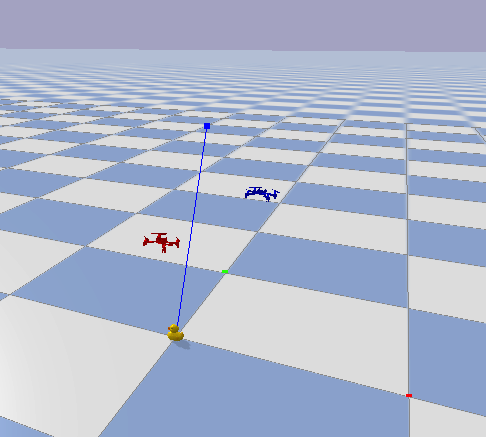
\includegraphics[height=5cm]{lib/graphics/drone_sim.png}
    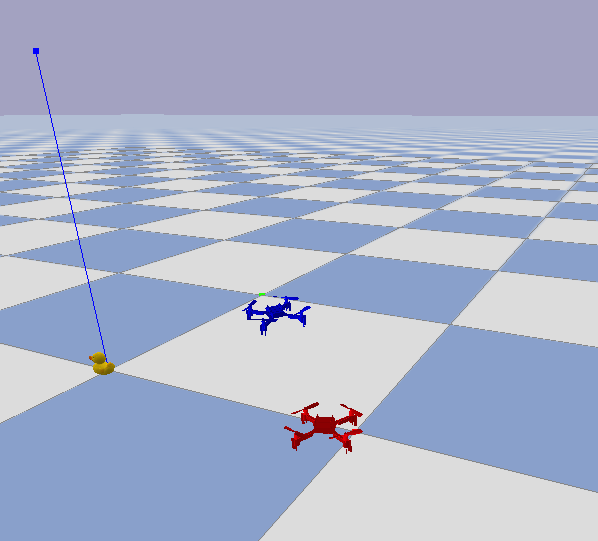
\includegraphics[height=5cm]{lib/graphics/drone_sim2.png}
    \caption[grafisches Modell der Simulation]{grafisches Modell der Simulation\footnotemark}
    \label{abb:simenv model}
\end{figure}
\footnotetext{Eigene Darstellung}


% Grundbasis der eigenen Simulation
Die Umsetzung, der zu Beginn dieses Kapitels beschriebenen Simulationsumgebung, basiert auf der Verwendung der Basissimulation und der Steuerungsklasse.
Zusätzlich sind teilweise Funktionen aus ähnlichen, bereits nativ vorhandenen Szenarien mit Änderungen übernommen und im Programm entsprechend gekennzeichnet.
Die beschriebene Simulation ist innerhalb einer Klasse nach dem Gymnasium Framework aufgebaut.
Zusätzlich wird die Simulation durch eine erbende Klasse umhüllt, um für den Algorithmus eine verarbeitbare Abstraktionsschicht zu erzeugen.
In dieser Schicht wird die Steuerung der angreifenden Drohne abstrahiert, sodass die Trainingsumgebung lediglich die Bestimmung einer Aktion für die verteidigende Drohne erwartet.
Nachfolgend wird die Umsetzung dieser beiden Klassen, nach den einzelnen Funktionen des Gymnasium-Frameworks erläutert.

% Init DualDrone Aviary
Die Simulation beider Quadrokopter ist in der Klasse \textbf{DualDroneAviary} definiert.
Zur Initialisierung einer Simulationsinstanz wird die \textbf{Init-Funktion} aufgerufen, welche die Übergabe aller simulationsrelevanten Parameter erwartet.
Die Parameter umfassen unter anderem Informationen zur Anzahl und Art und Position der Drohnen, gewählte Handlungs- und Beobachtungsarten sowie die unabhängigen Variablen der Trainingsszenarien.
Außerdem wird die Gewichtung der Belohnungsfunktion als Parameter entgegengenommen.
Kernaufgabe der Funktion ist die Umsetzung der Eigenschaften eines Trainings- und Testszenarios.
Dies beinhaltet u. A. die Erzeugung und Übermittlung der zufälligen Start- und Zielpunkte und des zufälligen Windeffektes mittels unterstützender Funktionen aus der eigenen Hilfsklasse.
Die verteidigende Drohne wird zufällig innerhalb von 1,5 Meter in X- und Y-Richtung und 0.1 bis 3 Meter in Z-Richtung zum Ursprung initialisiert.
Hingegen wird die angreifende Drohne im Rahmen von zwei bis sechs Metern uniform um den Ursprung herum auf einer möglichen Höhe von 0.1 bis fünf Meter platziert.
Sind die Eigenschaften bestimmt, können diese zur Erzeugung der darunter liegenden Abstraktionsschicht der BaseAviary Instanz genutzt werden.

% Observation Space
Der Beobachtungsraum in dieser Simulation wird durch einen Informationsvektor in der \textbf{ObservationSpace-Funktion} definiert.
Der für die Experimente eingesetzte Informationsvektor je Drohne enthält die Position, Fortbewegungsrichtung und Geschwindigkeit.
Die Position wird durch dreidimensionale Koordinaten, die Ausrichtung durch Quaternion und Drehwinkel kodiert.
Positionen können dabei von $- \inf$ bis $+ \inf$ in X- und Y-Richtung und von $0$ bis $+ \inf$ in Z-Richtung betrachtet werden.
Fortbewegungsrichtung und Geschwindigkeit werden als Geschwindigkeitsvektor von minus bis plus unendlich zu den Koordinatenachsen definiert.
Insgesamt ist für jede Drohne ein Beobachtungsvektor mit sechs Elementen innerhalb eines Wörterbuchobjektes definiert.

% Action Space
Die Definition des Aktionsraums ist in der \textbf{ActionSpace-Funktion} bestimmt.
Eine Aktion des ausgewählten Aktionstyps wird als vierdimensionaler Vektorbereich definiert.
Jeder Wert des Vektors besitzt eine untere und obere Grenze, aus dessen Bereich die endgültige Aktion gewählt wird.
Zur Steuerung des Quadrokopters wird im Rahmen dieser Arbeit der Aktionstyp auf Basis der Geschwindigkeit verwendet.
Der Wertebereich des Richtungsvektors ist dabei von $[-1,-1,-1]$ bis $[1,1,1]$ definiert. 
Das vierte Element spiegelt den Anteil der maximalen Geschwindigkeit von null bis eins wider.

% Step 
Ist eine Aktion regelbasiert oder durch ein RL-Modell bestimmt, wird diese als Parameter an die \textbf{Step-Funktion} weitergegeben.
Auf der Ebene der DualDroneAviary Klasse kann die übergebene Aktion in Abhängigkeit vom anfangs initialisierten Wind abgewandelt werden.
Der Windvektor wird in Abhängigkeit des Winkels zwischen Bewegungsrichtung der Drohne und des Windes zur Aktion hinzugefügt.
Der Drohnenbewegungsrichtung wird die Windrichtung addiert sowie die Geschwindigkeit in Abhängigkeit des Eintreffwinkels vollständig positiv, negativ oder gar nicht beeinflusst.
Anschließend wird unter veränderter oder unveränderter Aktion die Schrittfunktion der Elternklasse aufgerufen.
Die Schrittfunktion der Elternklasse übersetzt die Aktion aus dem Aktionsraum in konkrete Rotordrehzahlen und übt diese unter Einfluss der simulierten Physik aus.
Zur Erhöhung des Realismusgrades wird zusätzlich zu den Effekten der pybullet Physik-Engine ein Boden- und Trägheitseffekt eingesetzt.
Anschließend wird die neue Zustandsbeobachtung, die entstandene Belohnung, das Rücksetzkriterium und ein Datenobjekt für Zusatzinformationen zurückgegeben.

% Reward ?
Die Bestimmung der Belohnung ist unter der \textbf{reward-Funktion} der DualDroneAviary Klasse implementiert.
Innerhalb dieser Funktion werden aus dem aktuellen Zustand der Simulation Kennzahlen zu dessen Evaluation berechnet und gewichtet.
Durch die Gewichtung und die Optimierung dieser kann das Strategieziel formuliert und der Einfluss der einzelnen Kennzahlen angepasst werden.
Die Aufsummierung der Produkte aus den folgenden Kennzahlen und deren Gewichtung spiegelt die Belohnung zu jedem Zeitschritt wider:
\begin{itemize}
    \item Distanz zwischen der angreifenden und verteidigenden Drohne
    \item Belohnung bei erfolgreichem Abfangen der angreifenden Drohne
    \item Negative Belohnung, sofern die angreifende Drohne den Zielpunkt erreicht hat
    \item Belohnung für eine möglichst direkte Flugrichtung zur gegnerischen Drohne
    \item Lineare Belohnung der Geschwindigkeit
\end{itemize}
Eine Optimierung der Gewichte wurde durch ausgiebige Evaluation unterschiedlicher Gewichtskombinationen und Messen der entsprechenden Erfolgsrate erzielt.
Zu jedem Zeitschritt eintretende Belohnungen wurden aufgrund ihrer Häufigkeit in Fünfer-Schritten, außerordentliche Belohnungen in 10000er-Schritten untersucht.
Insgesamt sind daraus unter anderem folgende in Abbildung 9 dargestellte Log-Dateien entstanden, welche den Optimierungsprozess widerspiegeln.

\begin{figure}[htb]
    \centering
    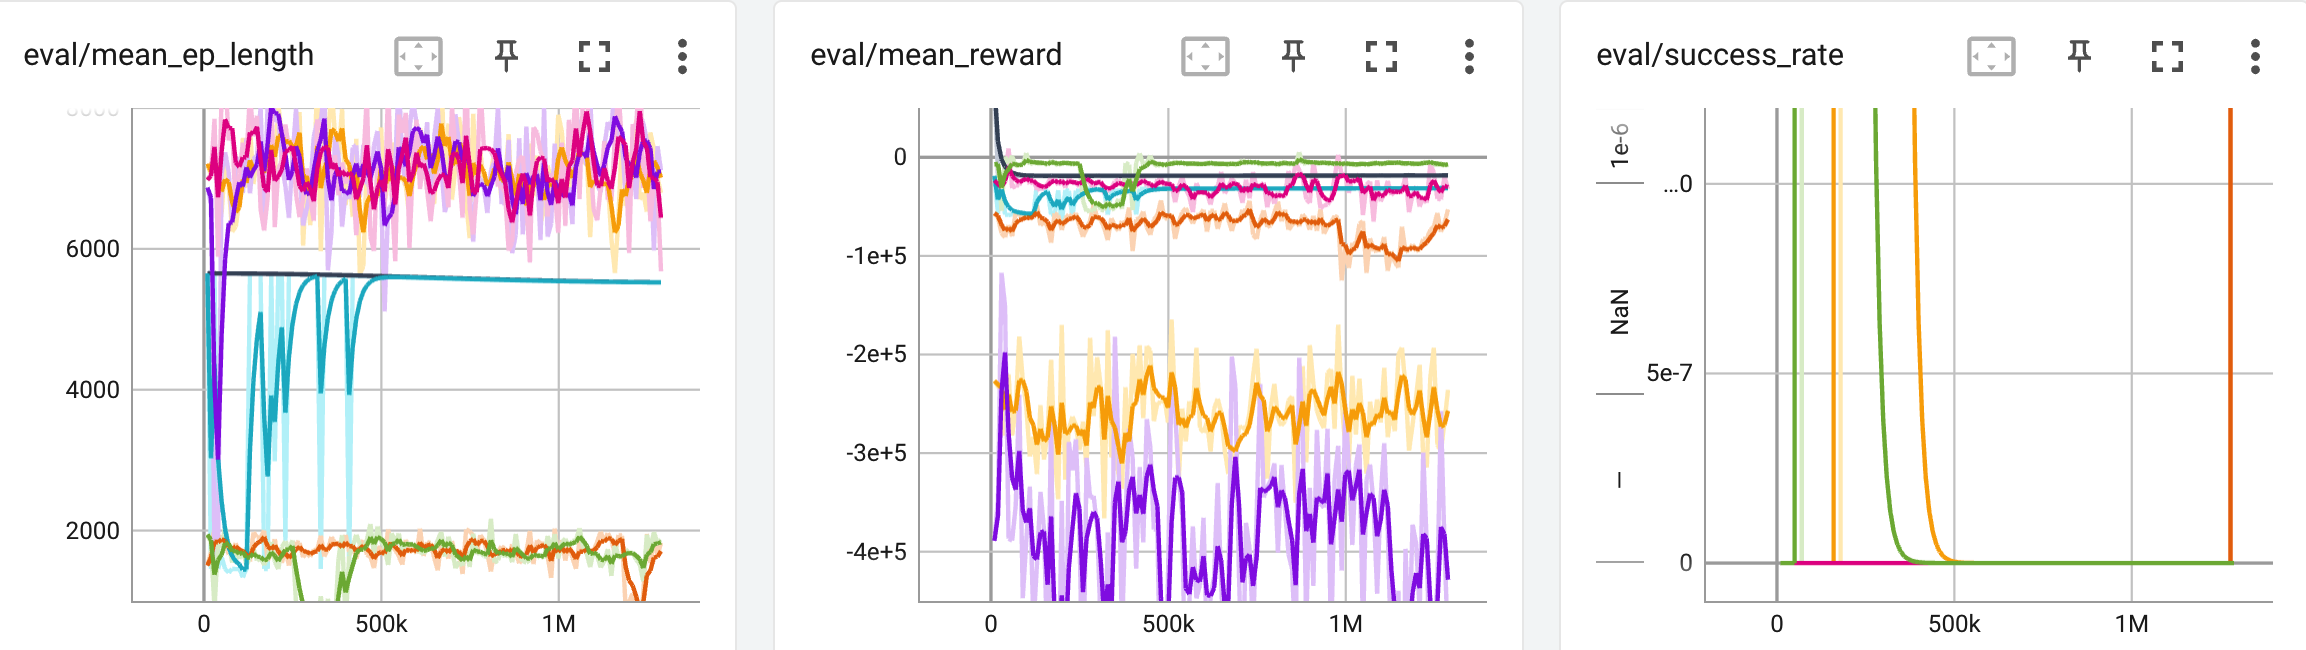
\includegraphics[height=4.5cm]{lib/graphics/speed_reward_logs.png}
    \caption[Episodenlänge, Belohnung und Erfolgsrate unter verschiedenen Gewichtungen]{Episodenlänge, Belohnung und Erfolgsrate unter verschiedenen Gewichtungen\footnotemark}
    \label{abb:reward-logs}
\end{figure}
\footnotetext{Diagramme durch die Tensorboard Bibliothek erstellt}

Die Optimierung der Belohnungsfunktion erzielte $[-10, 50000, 50000, 25, 20]$ als optimalen Gewichtsvektor, da hierunter mehrere Algorithmen wie PPO und A2C, eine positive Erfolgsrate verzeichneten.

% reset
Ist das Rücksetzkriterium erfüllt, wird die Simulationsumgebung mittels \textbf{reset-Funktion} neu gestartet.
Dabei werden neue Zufallspositionen der Drohnen und des Ziels sowie im vierten Trainingsszenario neue Windeigenschaften generiert.
Sind diese Variablen verändert, kann die Rücksetzfunktion der darunterliegenden Abstraktionsschicht aufgerufen werden.
Die Funktion der BaseAviary-Klasse setzt die Zeitschritte und die Drohneninformationen zurück und baut das grafische Modell neu auf.
Über den Zugriff auf den Klienten der pybullet Physik-Engine werden die Drohnenobjekte sowie das Untergrundobjekt aus den URDF-Dateien geladen und an entsprechenden Stellen platziert.
Zur Unterscheidung des verteidigenden Quadrokopters von der angreifenden Drohne werden zwei nahezu identische URDF-Dateien verwendet, welche sich nur in der Farbgebung zwischen rot und blau unterscheiden.
Am Ende der Funktion wird der erste Beobachtungsvektor der neuen Episode sowie ein Infoobjekt zurückgegeben.

% Defender Drone Wrapper und Attacker Drone Wrapper
Die zuvor beschriebene Klasse vererbt ihre Variablen und Funktionen auf die höhergelegenen Abstraktionsschichten der \textbf{DefenderDroneWrapper} und \textbf{AttackerDroneWrapper} Klasse.
Auf dieser Ebene bietet die Simulation ihre Schnittstelle für die Verwendung durch den IL- und RL-Algorithmus.
Dafür ist es notwendig, den Beobachtungsraum sowie den Aktionsraum neuzudefinieren.
Zur \textbf{Initialisierung} werden zum einen alle Parameter zur Instanziierung des DualDroneAviary Objekt erwartet.
Zum anderen sind zusätzlich die Strategie und dessen Rauschverhalten der nicht durch RL oder IL gesteuerten Drohne anzugeben, sodass diese in Klassenvariablen gespeichert werden.
Auf Ebene der Wrapper-Klassen wird der \textbf{Beobachtungsraum} mit allen Informationen beider Quadrokopter zu einem zwölf elementigen Vektor zusammengefasst.
Der \textbf{Handlungsraum} hingegen umfasst auf dieser Ebene lediglich einen vier-elementigen Vektor mit dem bekannten Wertebereich.
Zur Ausführung eines Simulationsschrittes werden in der \textbf{Step-Funtkion} die Aktion der jeweils gegnerischen Drohne und die durch das Modell übergebene Aktion in ein gemeinsames Datenobjekt überführt.
Anschließend kann mittels dieses Datenobjektes die Schrittfunktion der Elternklasse aufgerufen, und deren Rückgabewerte an den zu optimierenden Algorithmus weitergereicht werden.
Als \textbf{Belohnungswert} wird auf die im Trainingsszenario relevante Komponente des Belohnungsobjektes zugegriffen.

Werden die beschriebene Umsetzung der Simulationsumgebung zusammengefasst, kann folgendes Klassendiagramm und deren Funktionsabhängigkeiten in Abbildung 10 betrachtet werden.

\begin{figure}[htb]
    \centering
    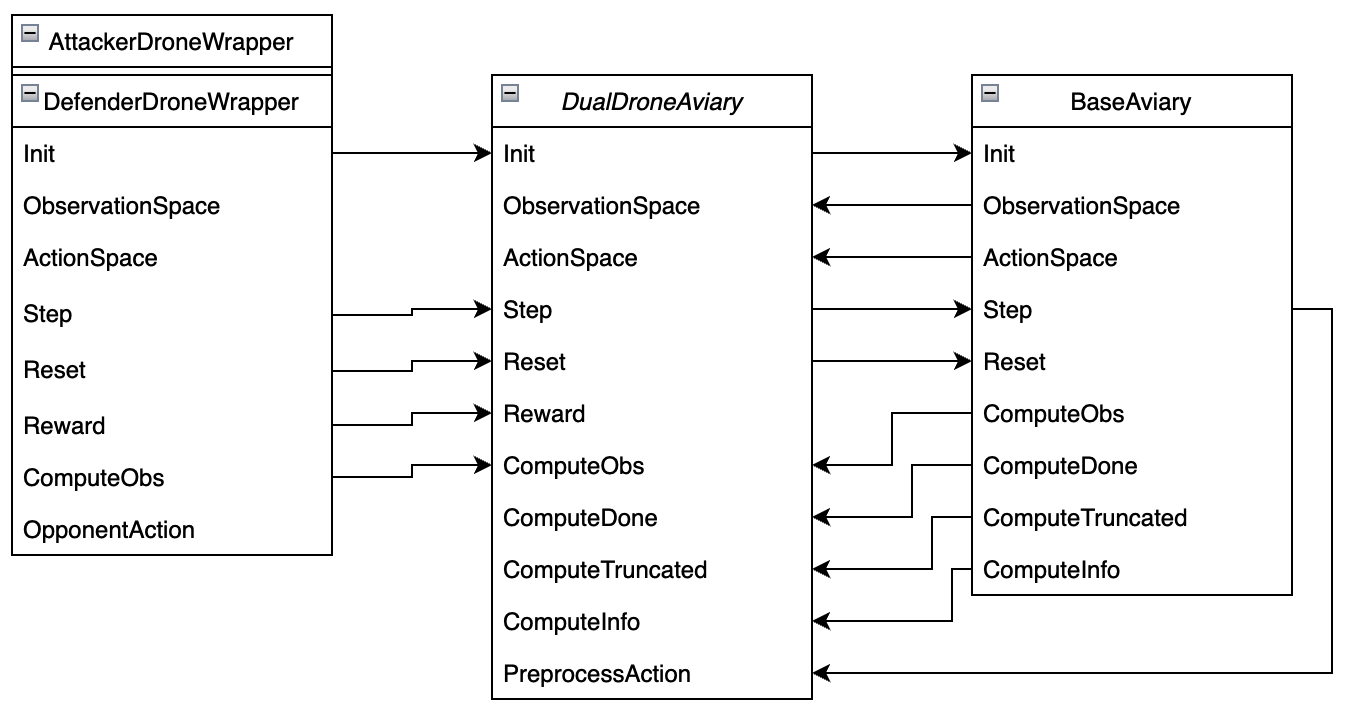
\includegraphics[height=6cm]{lib/graphics/simenv structure.png}
    \caption[Klassendiagramm mit Funktionsabhängigkeiten]{Klassendiagramm mit Funktionsabhängigkeiten\footnotemark}
    \label{abb:drone axis}
\end{figure}
\footnotetext{Eigene Darstellung}

\subsection{Programmumsetzung des Optimierungsverfahrens}

Mit der Entwicklung der Simulationsumgebung stehen Trainingsdaten zur Verfügung, um darauf aufbauend Strategien des verstärkenden Lernens zu optimieren.
Der gesamte Optimierungsprozess unterteilt sich in den Einsatz von imitierendem Lernen zu Beginn und folgender Optimierung mittels RL-Algorithmen. 
Die Umsetzung des Optimierungsverfahrens wird innerhalb der Python Dateien \textit{imitation\_train.py} und \textit{train.py} beschrieben.

Das imitierende Training beginnt mit dem Herstellen des Trainingsszenarios zum Akquirieren der Demonstrationen des Experten. 
Für die Erhebung der Trainingsdaten wird zunächst die Simulation unter den Trainingsgegebenheiten in 20000 Episoden ausgeführt.
Für das imitierende Lernen wurde der Parameter AGGR\_PHY\_STEPS der BaseAviary Klasse auf 50 gesetzt, was bedeutet, dass die Schrittfunktion nur alle 50 Zeitschritte aufgerufen wird und so je Episode deutlich weniger Aktionen erfolgen und Transitionen aufgezeichnet werden.
Damit verteilen sich die daraus entstehenden Transition-Objekt der verwendeten Softwarebibliothek Imitation, auf eine höhere Anzahl von verschiedenen Start- und Zielkoordinaten.
Das Transition-Objekt beschreibt einen durch die Aktion entstehenden Übergang vom bekannten zu einem neuen beobachteten Zustand sowie den Erhalt der Belohnung.
Hieraus ergeben sich eine Menge von aufeinanderfolgenden oder zeitversetzten Transition-Objekten.
Die Übergänge in den Trainingsdaten werden gemischt, so dass sie nicht entsprechend ihrer Entstehung geordnet liegen, um die Datenvielfalt innerhalb einzelner Batches zu erhöhen und korrelierende Effekte zu mindern. 
Basierend auf diesen Transaktionsdaten werden in 4000 Epochen die Gewichte der zu optimierenden Strategie angepasst.
Die Anpassung der Gewichte einer Akteur-Kritiker-Strategie wird durch den Behavioral Cloning Algorithmus vorgenommen.
Dessen Ziel ist es, mittels eines neuronalen Netzes eine Funktion von einem beobachteten Zustand zu der vom Experten gewählten Aktion zu approximieren.

Als Experte wird eine regelbasierte Version der jeweils zu optimierenden Strategie eingesetzt.
Alle regelbasierten Strategien sind in der \textit{rule-based.py} Datei deklariert und umfassen eine regelbasierte Strategie für die verteidigende Drohne sowie die Trainings- und Testversion der anzugreifenden Drohne.
Die verteidigende Drohne verfolgt regelbasiert die direkte Flugbahn zu einem Vorhaltepunkt in Bewegungsrichtung der Angreiferdrohne.
Der Vorhaltepunkt rückt mit geringer werdender Distanz zur generischen Drohne immer näher zu dessen aktueller Position.
Die angreifende Drohne wird im ersten Trainingsszenario regelbasiert gesteuert, indem sie sich von ihrem Startpunkt in gerader Fluglinie zum Zielpunkt begibt.
Dessen Erweiterung zur parabelförmigen Fluglinie wird in der nachfolgenden Sektion der Umsetzung des Laborexperiments behandelt. 

Wurde ein Akteur-Kritiker Modell durch imitierendes Lernen hin zum regelbasiertem Verhalten optimiert, wird dieses als Basis zur weiteren Optimierung mittels RL verwendet.
Im RL-Prozess ist zu beachten, dass anders als beim imitierenden Lernen zu jedem Zeitschritt eine neue Aktion gewählt wird, da der Parameter AGGR\_PHY\_STEPS hier standardmäßig bei 1 liegt.
Mit dem Einsatz des \textit{train.py} Programms lässt sich das in einer Pickle-Datei gespeicherte Modell laden.
Dazu wird das grundlegende neuronale Netz des PPO-Objekts  mit derselben Architektur und den trainierten gewichten des Modells aud dem imitierenden Lernen initialisiert.
Anschließend werden die Gewichte und Vorurteile in ein Objekt des PPO-Algorithmus von Stable-Baselines3 übertragen.
Mittels der learn-Funktion kann die erzeugte Strategie im gegebenen Trainingsszenario über eine Anzahl von Zeitschritten weiter optimiert werden.
Die während des RL Prozesses verwendeten Trainingszeitschritte lagen bei 2,592,000, welche sich aus der Trainingszeit von 180 Minuten und der Simulationsfrequenz von 240 Schritten pro Sekunde zusammensetzen.
Durch die Tensorboard Bibliothek werden während des Trainingsprozesses gemittelte Metriken über alle Episoden berechnet sowie alle 10000 Zeitschritte eine Evaluation durchgeführt.
In der Evaluationsperiode wird die aktuelle Strategie bemessen und deren Episodenlänge, erzielte Belohnung und Erfolg aufgezeichnet.
Als erfolgreich wird die Simulation gekennzeichnet, sobald die Strategie der Verteidigerdrohne die angreifende Drohne durch Kollision abfangen konnte.
Nach dem Abschluss der Optimierung werden die neuen Modelle in Pickle Dateien gespeichert. 

\subsection{Programmumsetzung des Laborexperiments}

Als letzter Teil der Umsetzung wird die Durchführung des Experiments betrachtet.
Kernaufgabe dieses Teils ist die Erhebung und Auswertung der Messdaten entsprechend des in der Einleitung des Kapitels verfassten Experimentaufbaus.
Die Erhebung der Testdaten erfolgt durch das \textit{test.py}, die Auswertung durch das \textit{experiment\_evaluation.py} Skript.

Mit der Ausführung des ersten Skripts wird eine Testklasse instanziiert und die Simulation nach den Eigenschaften des Testszenarios erzeugt.
Das Testszenario implementiert die Anforderung der Randomisierung des Zielpunktes.
Zur zufälligen Bestimmung des Zielpunkts wird, ebenso wie zur Initialisierung der Verteidigerdrohne, eine uniforme Verteilung bis zu 1,5 Meter um den Ursprung verwendet.
Eine uniforme Verteilung fördert dabei die Varianz der Testszenarien und erhöht so die Validität des Experiments.
Anders als bei der Initialisierung der Drohnen wird die Höhe des Zielpunktes stets auf 0,5 Meter festgelegt, um so Bodenkontakt und Simulationserfolg abzugrenzen.
Zusätzlich zur Randomisierung des Zielpunktes wird im Testszenario der regelbasierte angreifende Quadrokopter im Aspekt seiner parabelförmigen Anflugsstrategie verändert.
Ausgehend von den Startkoordinaten des Angreifers werden dazu insgesamt fünf Wegpunkte entlang einer unten geöffneten Parabel berechnet, welche nacheinander angeflogen werden.
Die Parameter der Parabel berechnen sich wie in den Formeln 8 bis 10 dargestellt.

\begin{description}
    \item \begin{center} $ a = -1 / (2 * ($Distanz zum Zielpunkt$ / 6))$ (8)\end{center}
    \item \begin{center} $ b = 0$ (9)\end{center}
    \item \begin{center} $ c = $ Z-Koordinate des Startpunktes (10)\end{center}
\end{description}

Alle Messdaten werden aus der hundertfachen Durchführung der Testsimulation erhoben.
Zu jedem Zeitschritt jeder Episode wird durch das RL-Modell eine bestimmte Aktion ausgeübt und eine Teilmenge des daraus resultierenden Zustands gemessen.
Die Teilmenge umfasst die durch die Aktion unmittelbar ausgelöste Belohnung und einen Wahrheitswert, ob mit Aktion ein Misserfolg der Simulation eingegangen wurde.
Beide Werte werden gekennzeichnet mit der jeweiligen Episode und dem Zeitschritt, in einer Tabelle als Datensatz hinzugefügt.
Nach dem erfolgreichen Durchlaufen aller Zeitschritte der 100 Episoden wird die Tabelle als Komma separierte Wertedatei (CSV) gespeichert.

Die erstellte Datei wird anknüpfend mittels \textit{experiment\_evaluation.py} ausgewertet, indem die Messdaten geladen, die Signifikanztests durchgeführt und jeweils ein Wahrheitswert für die Annahme/Ablehnung der Hypothesen bestimmt wird.
Für jeden dieser drei Schritte wurde eine Funktion entwickelt, welche im Skript aufgerufen wird.
Zum Laden der Messdaten sind die Speicherpfade zweier Wertedateien anzugeben, woraufhin der Verlauf der Kennzahlen zu einzelnen Episoden aggregiert werden.
Dabei wird zunächst die Episodenlänge, die kumulierte Belohnung und der final vorliegende Erfolgszustand ermittelt.
Basierend darauf kann die quadrierte absolute Abweichung der Belohnung je Episode zu dem Mittel aller kumulierten Belohnungen im Testprozess berechnet werden.
Nach dem Laden und Vorverarbeiten entspricht der Aufbau der Messdaten zweier Tabellen ähnlich der Tabelle Sechs.

\begin{table}[]
    \centering
    \begin{tabular}{lllll}
    Episode & Episodenlänge & \begin{tabular}[c]{@{}l@{}}kumulierte \\ Belohnung\end{tabular} & \begin{tabular}[c]{@{}l@{}}Belohnungsabweichung \\ zum Mittelwert\end{tabular} & Episodenmisserfolg \\
    1 & 1931 & 13512 & 3192 & 0 \\
    2 & 1579 & 8413 & 1873 & 1 \\
    3 & 1431 & 16920 & 6308 & 0 \\
    4 & 1944 & 6741 & 3701 & 1 \\
    5 & 1508 & 10173 & 89 & 0
    \end{tabular}
    \caption[Beispieltabelle der erhobenen aggregierten Messdaten]{Beispieltabelle der erhobenen aggregierten Messdaten}
\end{table}
\footnotetext{Eigene Darstellung}

Im nächsten Schritt ist mittels statistischer Signifikanztests die Ähnlichkeit zu einer Normalverteilung sowie die ungleiche Verteilung und mögliche Verbesserung aller Metriken zu untersuchen.
Die Implementierung der Signifikanztests wird im Rahmen dieser Arbeit durch die Softwarebibliothek SciPy bereitgestellt.
Iterativ werden für alle Metriken beider Messtabellen die Ähnlichkeit zur Normalverteilung überprüft, um zwischen einem T-Test und einem Mann-Whitney U Test auszuwählen.
Anschließend wird je Metrik der entsprechende Test zur Ungleichheit und Verbesserung der Verteilung ausgeführt, woraus je Test eine Teststatistik und ein P-Wert gespeichert wird.
Liegt der P-Wert eines Tests unter dem Signifikanzniveau von 10 \% wird die H0 Hypothese abgelehnt und daraus schlussfolgernd die Ungleichheit oder Verbesserung der Metrik angenommen.
Insgesamt wird diese Auswertung der Leistungsdaten zweier Strategien zweimal durchgeführt.
Dabei werden die erzielten Messdaten zwischen den Strategien aus Trainingsszenario eins und drei sowie aus Szenario eins und vier verglichen.
Der vollständige Prozess des Experiments kann auch als BPMN Modell wie in Abbildung 11 dargestellt werden. 

\begin{figure}[htb]
    \centering
    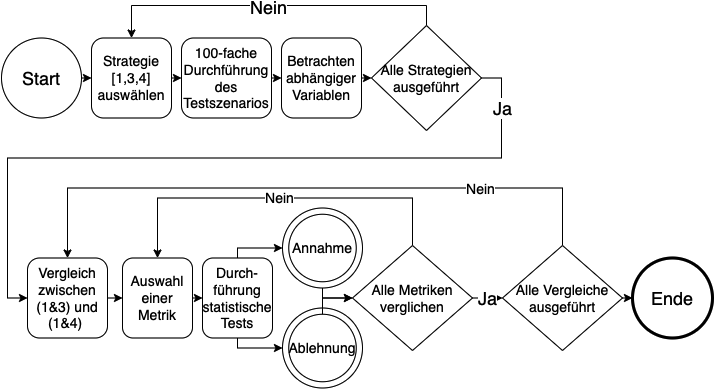
\includegraphics[height=6cm]{lib/graphics/experimentflow.png}
    \caption[BPMN Prozess des Laborexperiments]{BPMN Prozess des Laborexperiments\footnotemark}
    \label{abb:experiment flow}
\end{figure}
\footnotetext{Eigene Darstellung}